\chapter{Systembeskrivelse}
	Systemet består af en database med brugeradgang via iOS applikation.
	Databasen indeholder brugere, projekter, PDF tegninger og data om projekterne.
	Et projekt indeholder en PDF tegning, tegne objekter, mulighed for upload af billede og tekst.
	
	\begin{figure}[H]
		\centering
		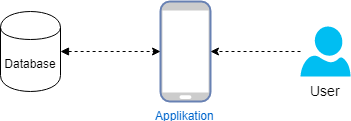
\includegraphics[width=0.4\linewidth]{Systembeskrivelse/Oversigtoversystem}
		\caption{Oversigt over systemet}
		\label{fig:OversigtSystembeskrivelse}
	\end{figure}
	
	Systemet skal kunne håndtere de bygge projekter Rambøll har, og oprette nye når de overtager et nyt bygge projekt.
	Disse skal kunne tilgåes af Rambøll ansatte, via enten en smartphone eller tablet.
	Rambøll ansatte får tildelt et personligt login.
	Brugere skal kunne oprette en registring for et givet projekt.
	Når en bruger er færdig med at oprette sin registrering, skal denne kunne exportes til en excel fil og sendes som en vedhæftet fil i en mail.
	Systemet har en log, som indeholder en liste over alle registreringer, til et givent projekt. \\	
				 
	\clearpage